
\section{Solution}
\subsection{Aufgabe 1}

2. Die Histogramme sind in Abbildung \ref{fig:2} dargestellt.

\begin{figure}
      \begin{subfigure}[b]{0.5\textwidth}
        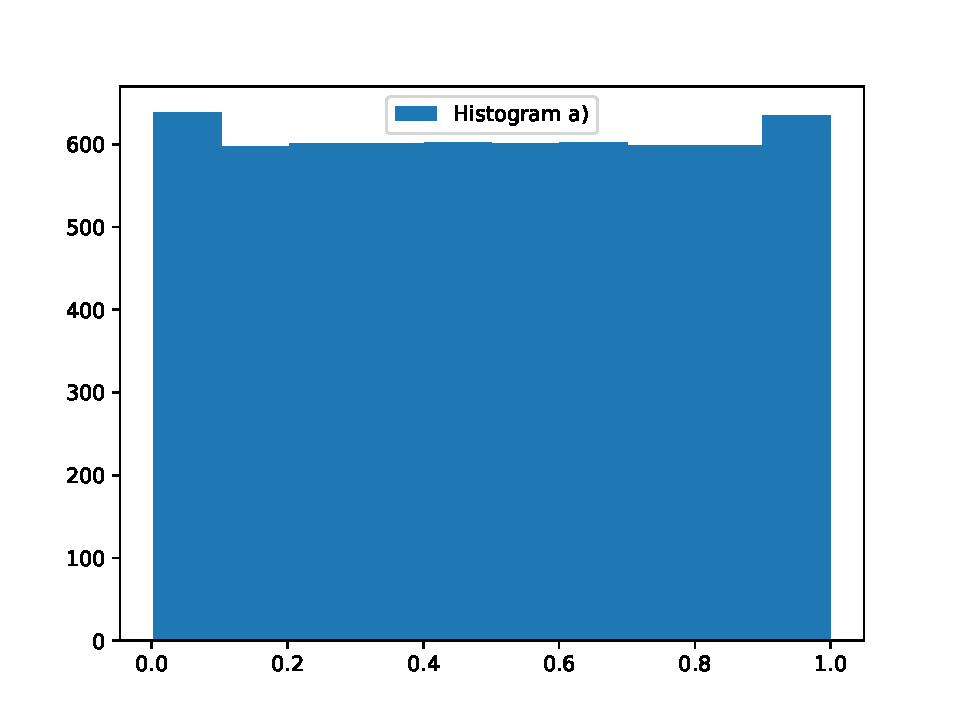
\includegraphics[width=\textwidth]{images/a.pdf}
        \caption{a)}
      \end{subfigure}
      %
      \begin{subfigure}[b]{0.5\textwidth}
        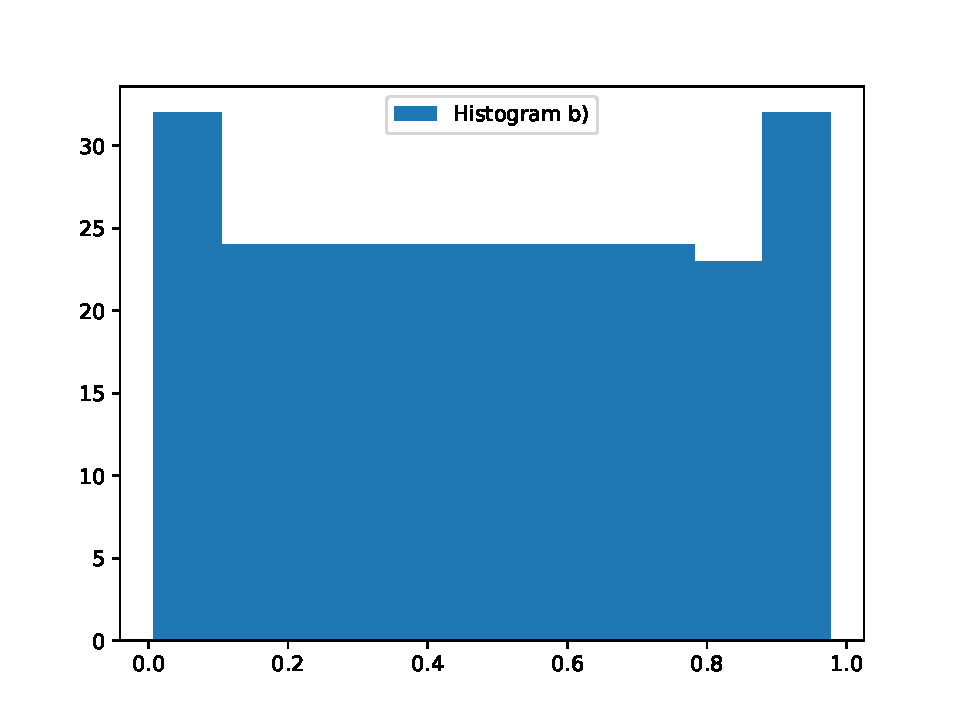
\includegraphics[width=\textwidth]{images/b.pdf}
        \caption{b)}
      \end{subfigure}
      \begin{subfigure}[b]{0.5\textwidth}
        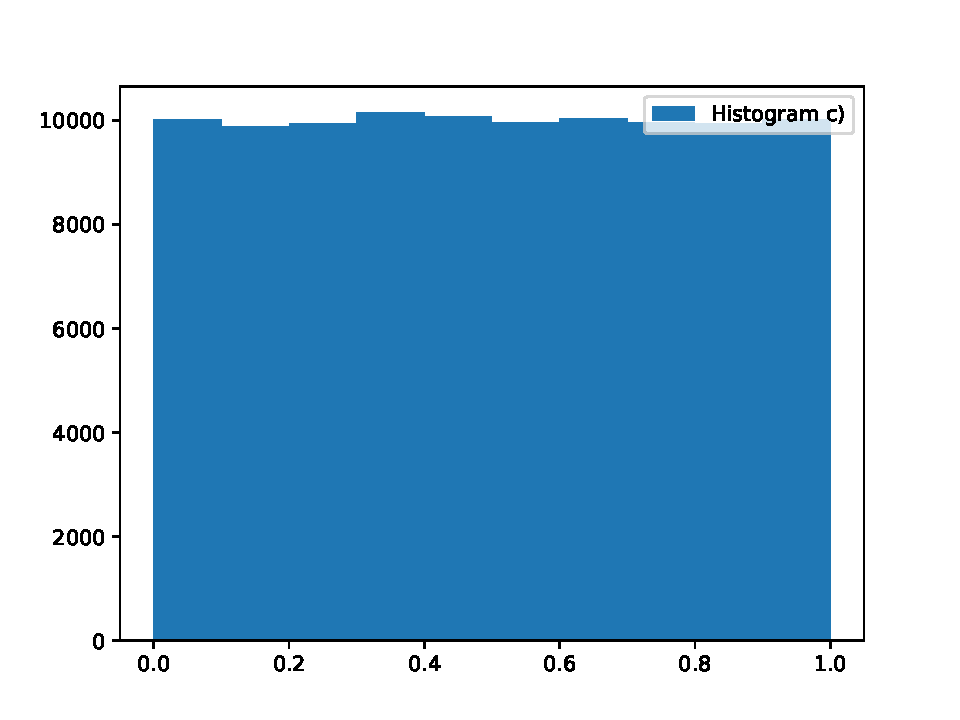
\includegraphics[width=\textwidth]{images/c.pdf}
        \caption{c)}
      \end{subfigure}
      %
      \begin{subfigure}[b]{0.5\textwidth}
        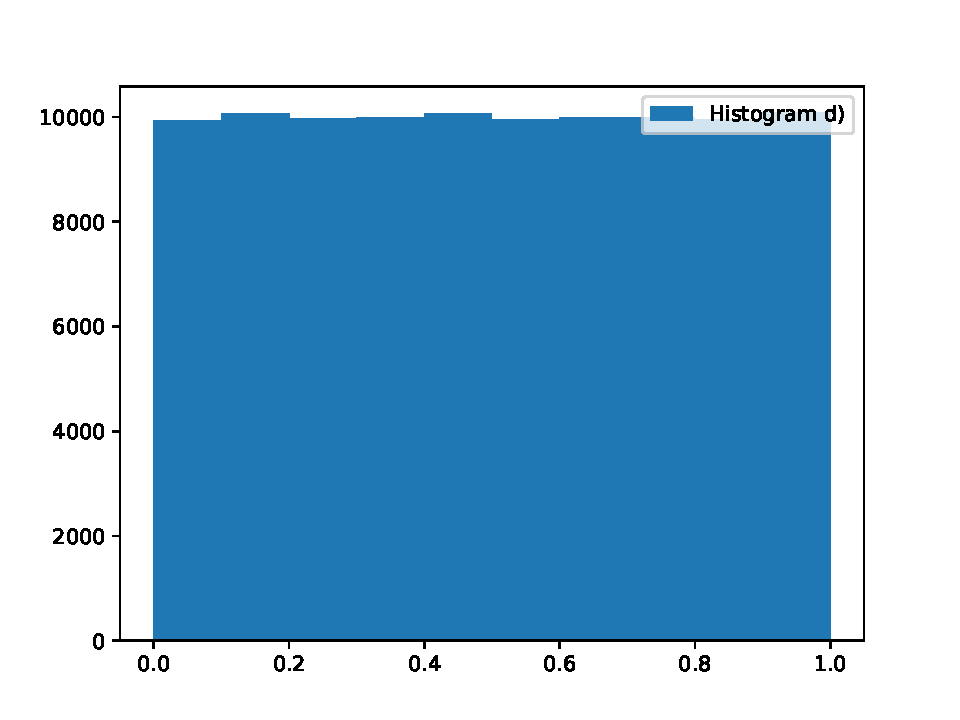
\includegraphics[width=\textwidth]{images/d.pdf}
        \caption{d)}
      \end{subfigure}
      \caption{Histogramme aus 2.}
      \label{fig:2}
    \end{figure}

    3. Die Zufallszahlen werden in Scatterplots aufgetragen. Bei a) und b) lässt sich eine klare Korrelation feststellen. 
    Dies ist ein unerwünschter Nachteil der Linear-Kongruent-Generatoren.
    Bei c) und d) wird nur jedes 10te Wertepaar geplottet, da die Abbildung recht groß ist. Dort ist keine so klare Korrelation zu erkennen.
    Aus der Vorlesung jedoch wissen wir, dass bei einer 3d Darstellung, diese Korrelation klarer zum vorschein kommt.
    

    \begin{figure}
        \begin{subfigure}[b]{0.5\textwidth}
          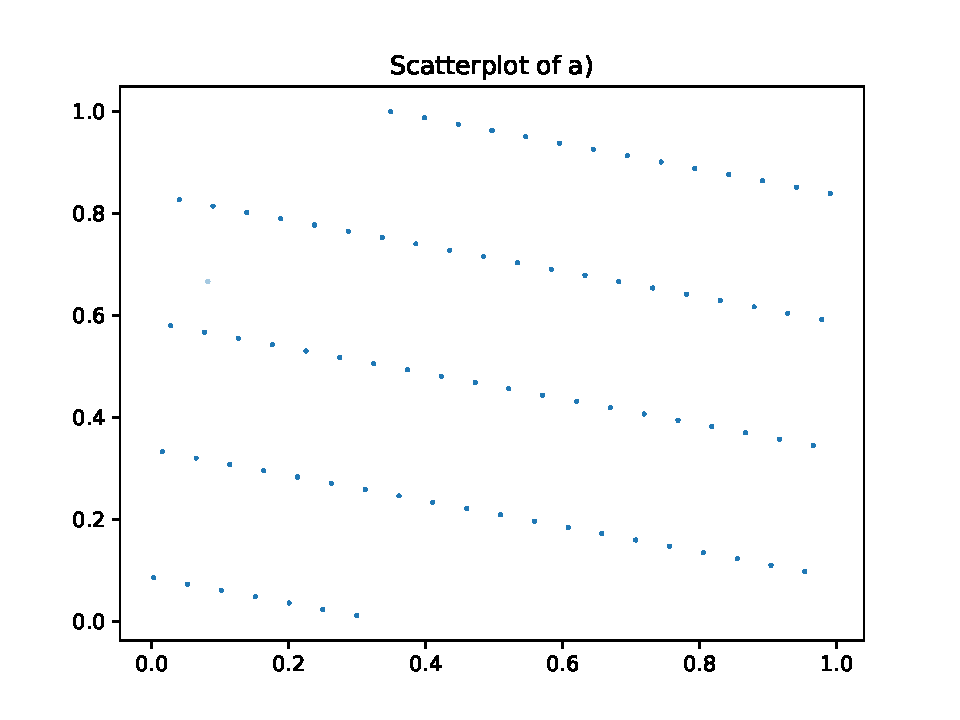
\includegraphics[width=\textwidth]{images/a2d.pdf}
          \caption{a)}
        \end{subfigure}
        %
        \begin{subfigure}[b]{0.5\textwidth}
          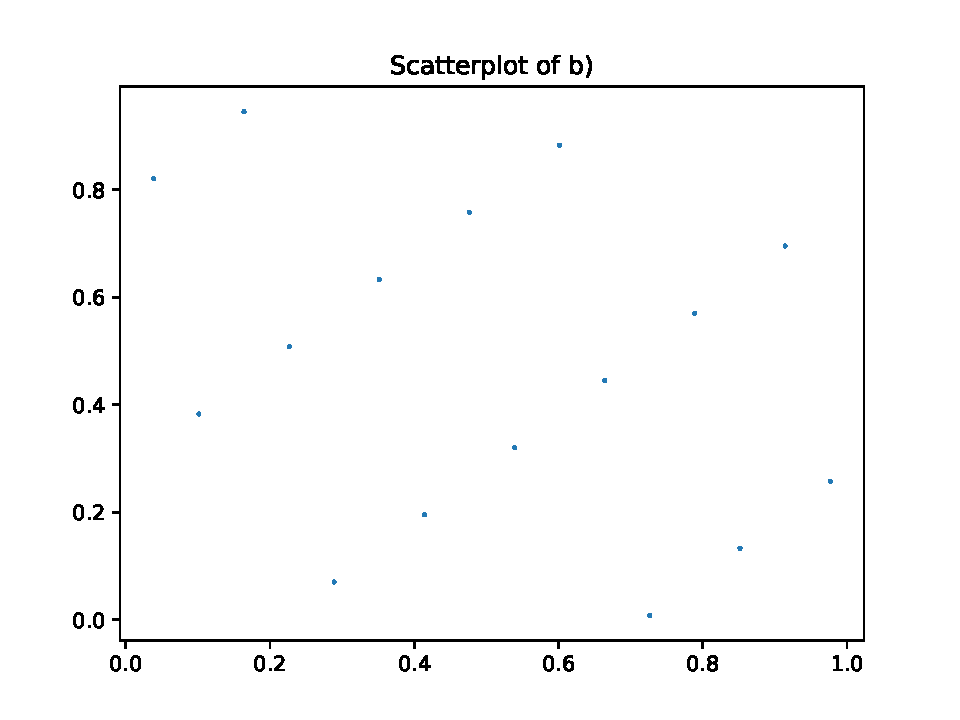
\includegraphics[width=\textwidth]{images/b2d.pdf}
          \caption{b)}
        \end{subfigure}
        \begin{subfigure}[b]{0.5\textwidth}
          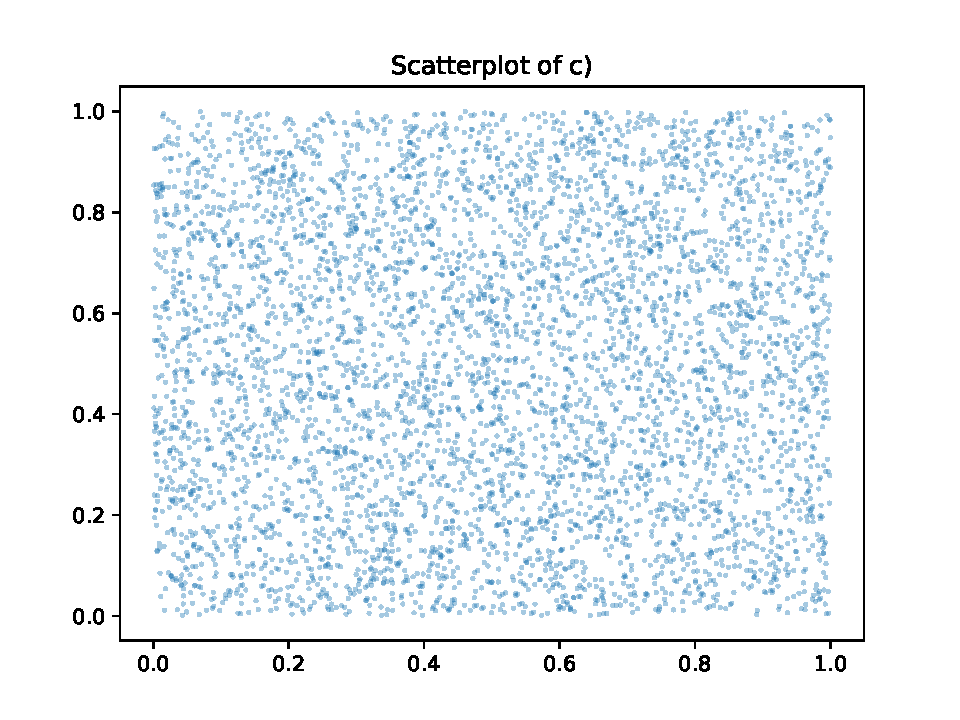
\includegraphics[width=\textwidth]{images/c2d.pdf}
          \caption{c)}
        \end{subfigure}
        %
        \begin{subfigure}[b]{0.5\textwidth}
          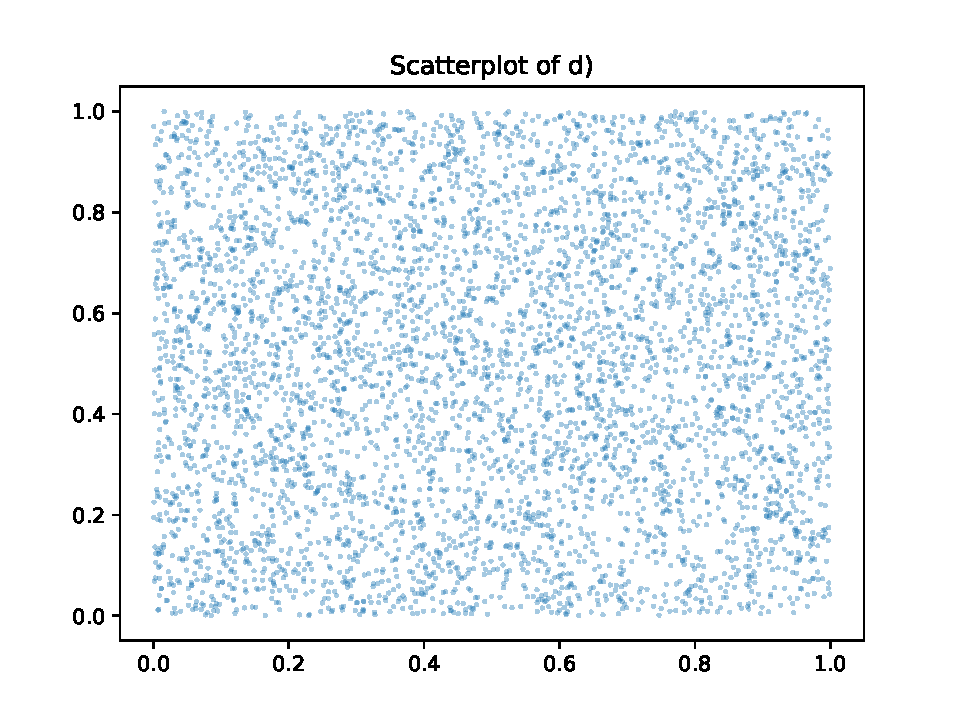
\includegraphics[width=\textwidth]{images/d2d.pdf}
          \caption{d)}
        \end{subfigure}
        \caption{Scatterplots of 3.}
        \label{fig:3}
      \end{figure}


\label{sec:auswertung}
